\documentclass[border=4pt]{standalone}
\usepackage{tikz}
\definecolor{cB1}{HTML}{DCE6F2}\definecolor{cB2}{HTML}{F8EADB}\definecolor{cI}{rgb}{0,0.45,0}
\definecolor{tB1}{HTML}{3E5C8A}\definecolor{tB2}{HTML}{A0522D}
\begin{document}
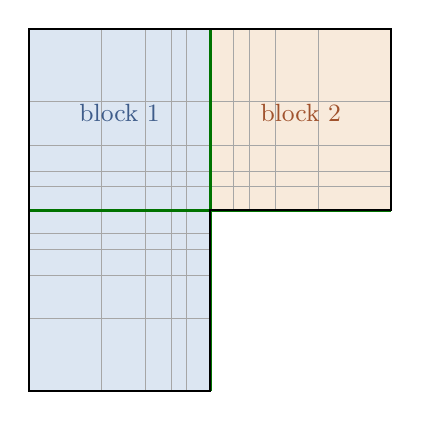
\begin{tikzpicture}[scale=4.6]
% L-shape: (0,1)^2 minus Q=[1/2,1]x[0,1/2]
\fill[cB1] (0,0) rectangle (0.5,1);
\fill[cB2] (0.5,0.5) rectangle (1,1);
% knot lines graded toward the re-entrant corner (geometric, ratio 0.6, 5 per block)
\def\knotsL{0.5-0.5*0.6^1,0.5-0.5*0.6^2,0.5-0.5*0.6^3,0.5-0.5*0.6^4}
\def\knotsR{0.5+0.5*0.6^1,0.5+0.5*0.6^2,0.5+0.5*0.6^3,0.5+0.5*0.6^4}
\foreach \x in \knotsL {\draw[black!35,line width=0.3pt] ({\x},0)--({\x},1);}
\foreach \x in \knotsR {\draw[black!35,line width=0.3pt] ({\x},0.5)--({\x},1);}
\foreach \y in \knotsL {\draw[black!35,line width=0.3pt] (0,{\y})--(0.5,{\y});}
\foreach \y in \knotsR {\draw[black!35,line width=0.3pt] (0,{\y})--(1,{\y});}
% interfaces x=0.5 and y=0.5 (green)
\draw[cI,line width=1.0pt] (0.5,0)--(0.5,1);
\draw[cI,line width=1.0pt] (0,0.5)--(1,0.5);
% boundary
\draw[black,line width=0.8pt] (0,0)--(0.5,0)--(0.5,0.5)--(1,0.5)--(1,1)--(0,1)--cycle;
\node[tB1,font=\small] at (0.25,0.77) {block 1};
\node[tB2,font=\small] at (0.75,0.77) {block 2};
\end{tikzpicture}
\end{document}
